% Copyright 2019 Clara Eleonore Pavillet

% Author: Clara Eleonore Pavillet
% Description: This is an unofficial Oxford University Beamer Template I made from scratch. Feel free to use it, modify it, share it.
% Version: 1.0

\documentclass{beamer}
\usepackage{pdfpages}
% Load Packages
\usepackage[utf8]{inputenc}
\usepackage{xcolor}
\usepackage{tikz}
\usetikzlibrary{positioning,calc}
\usepackage{graphicx}
\usepackage{hyperref}
\usepackage{amsmath}
\usepackage{listings}
\usepackage{fontawesome}
\usepackage[T2A]{fontenc}
\usepackage[utf8]{inputenc}
\usepackage[russian]{babel}

% Define Commands
\newcommand*{\ClipSep}{0.06cm} %To adjust footer logo
\newcommand{\E}{\mathrm{e}\,} %\def\I{e} % used to defined e for exp(x), see later what it should be
\newcommand{\ud}{\mathrm{d}}
\lstset{numbers=left, numberstyle=\tiny, stepnumber=1,firstnumber=1,breaklines=true,
    numbersep=5pt,language=Python,
    stringstyle=\ttfamily,
    basicstyle=\footnotesize, 
    showstringspaces=false
}

\usetheme{oxonian}
\usepackage{wrapfig}
\usepackage{listings}

\title{Въведение в OpenMP.}
\subtitle{\textit{Курс „Паралелно програмиране“}}
\titlegraphic{{
\includegraphics[width=5.3cm]{iaps.png}}} 

\author{\newline \newline Стоян Мишев}

\vspace{1cm}

\date{} %\today

\begin{document}
\lstset{language=Python}
{\setbeamertemplate{footline}{} 
\frame{\titlepage}}


\section*{План}\begin{frame}{План}\tableofcontents\end{frame}

%%%%%%%%%%%%%%%%%%%%%%%%%%%%%%%%%%%%%

\begin{frame}{Определение на OpenMP}

  \url{https://www.openmp.org/}
  
  \textbf{Стандарт} за писане на програми за създаване и управление на нишки. \pause

  Има варианти за С, С++, Фортран и др. \pause

  \textbf{Нишка} е част от програма, която има достъп до \textit{собствена} част от паметта, както и до общи ресурси за компютъра - памет, външни устройства, мрежа и т.н. \pause

  Лекцията е на основата на клипа \url{https://www.youtube.com/watch?v=IsBgW7-yldA}
  
\end{frame}


\begin{frame}{Версии на OpenMP}
  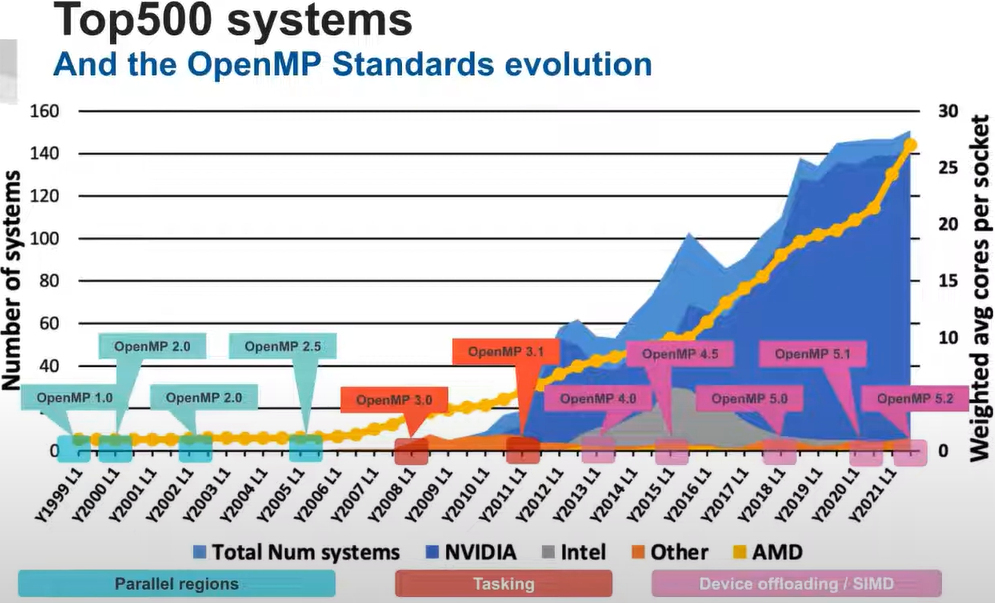
\includegraphics[width=\textwidth]{openmp-standards.png}
\end{frame}

\begin{frame}{Версии на OpenMP}
  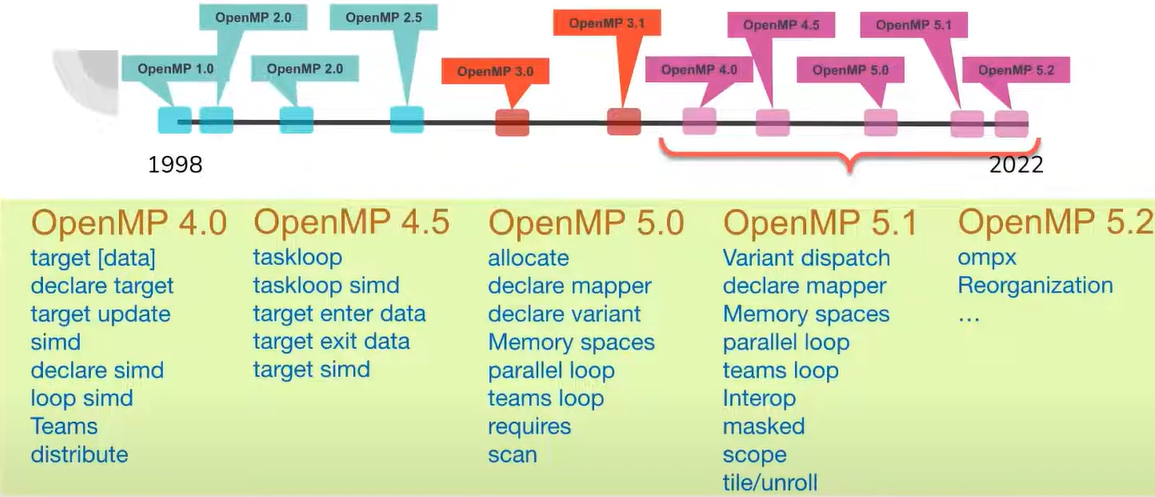
\includegraphics[width=\textwidth]{openmp-variants.png}
\end{frame}

\begin{frame}{Създаване и \textit{обединяване} на нишки}
  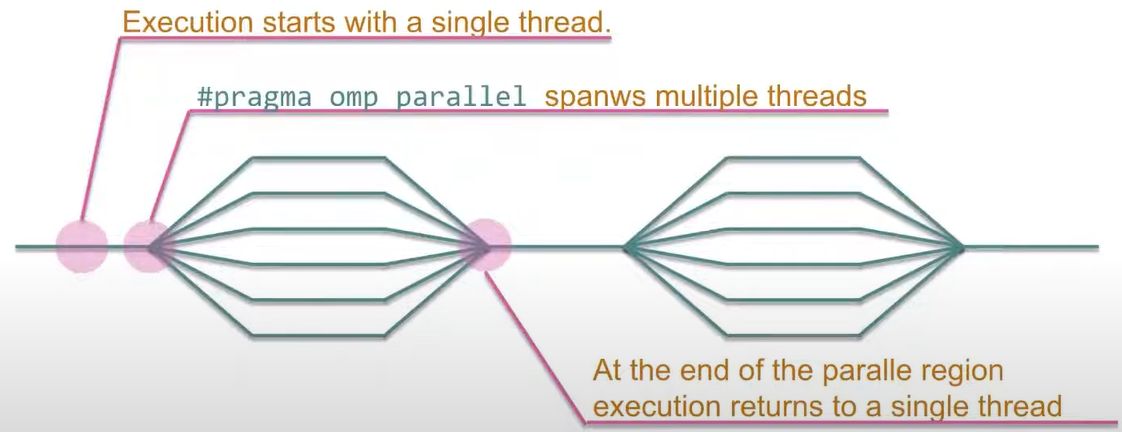
\includegraphics[width=\textwidth]{fork-join.png}
\end{frame}

\begin{frame}[fragile]{Създаване на нишки}
  
    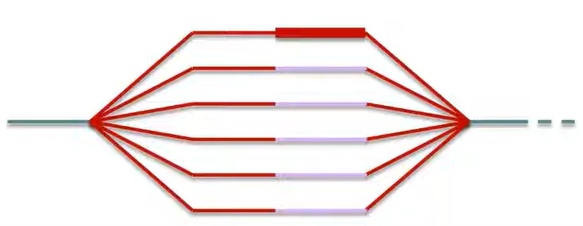
\includegraphics[width=0.8\textwidth]{master-thread}
    \begin{lstlisting}
      #pragma omp parallel{
        printf("hi from %d\n", omp_get_num_thread());

        #pragma omp master{
          printf("This shows once \n");
        }

      }
    \end{lstlisting}
\end{frame}

\begin{frame}{Хардуерни възможности и софтуерна абстракция}
  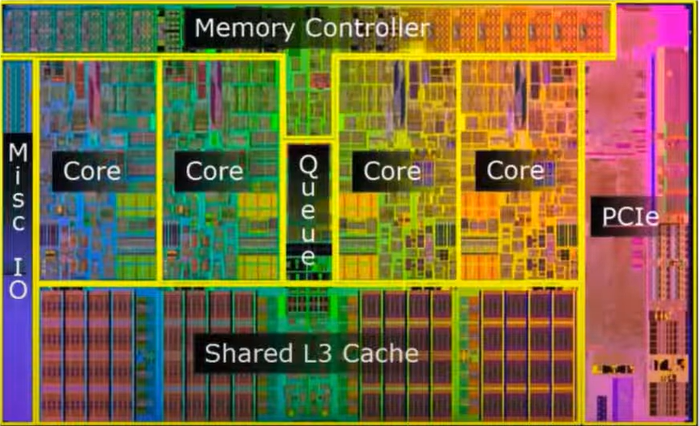
\includegraphics[width=\textwidth]{soft-hard}
\end{frame}

\begin{frame}[plain]{Хардуерни възможности и софтуерна абстракция}
  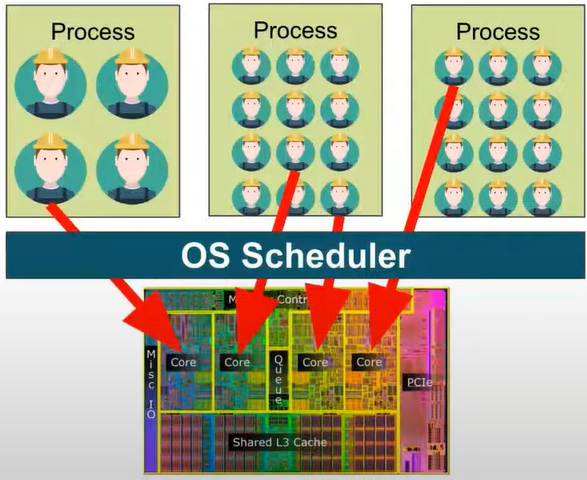
\includegraphics[width=\textwidth]{soft-hard1}
\end{frame}

\begin{frame}{Една и много нишки}
  \centering
  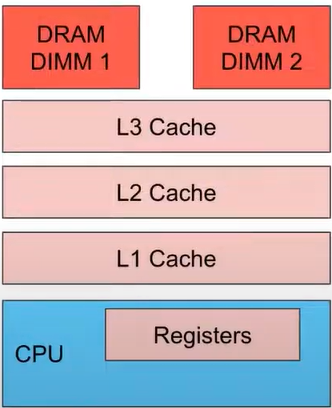
\includegraphics[width=0.2\textwidth]{single-thread}  \pause

  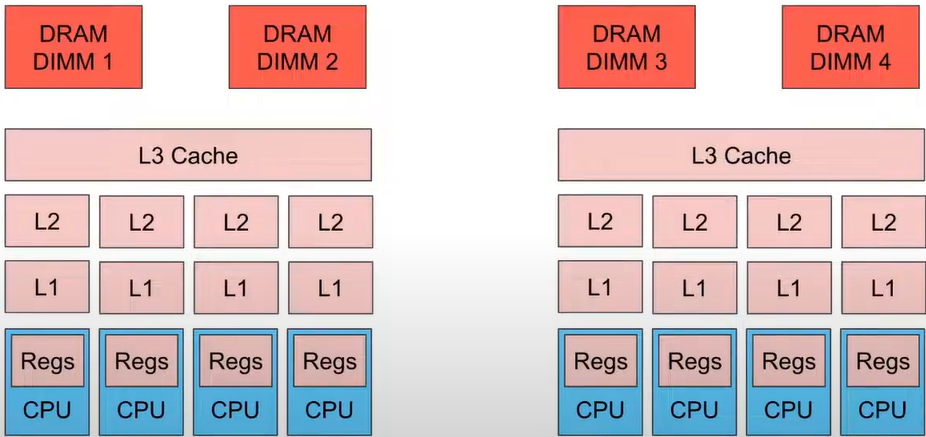
\includegraphics[width=0.6\textwidth]{multi-thread.png}  

\end{frame}


\begin{frame}{Shared}
  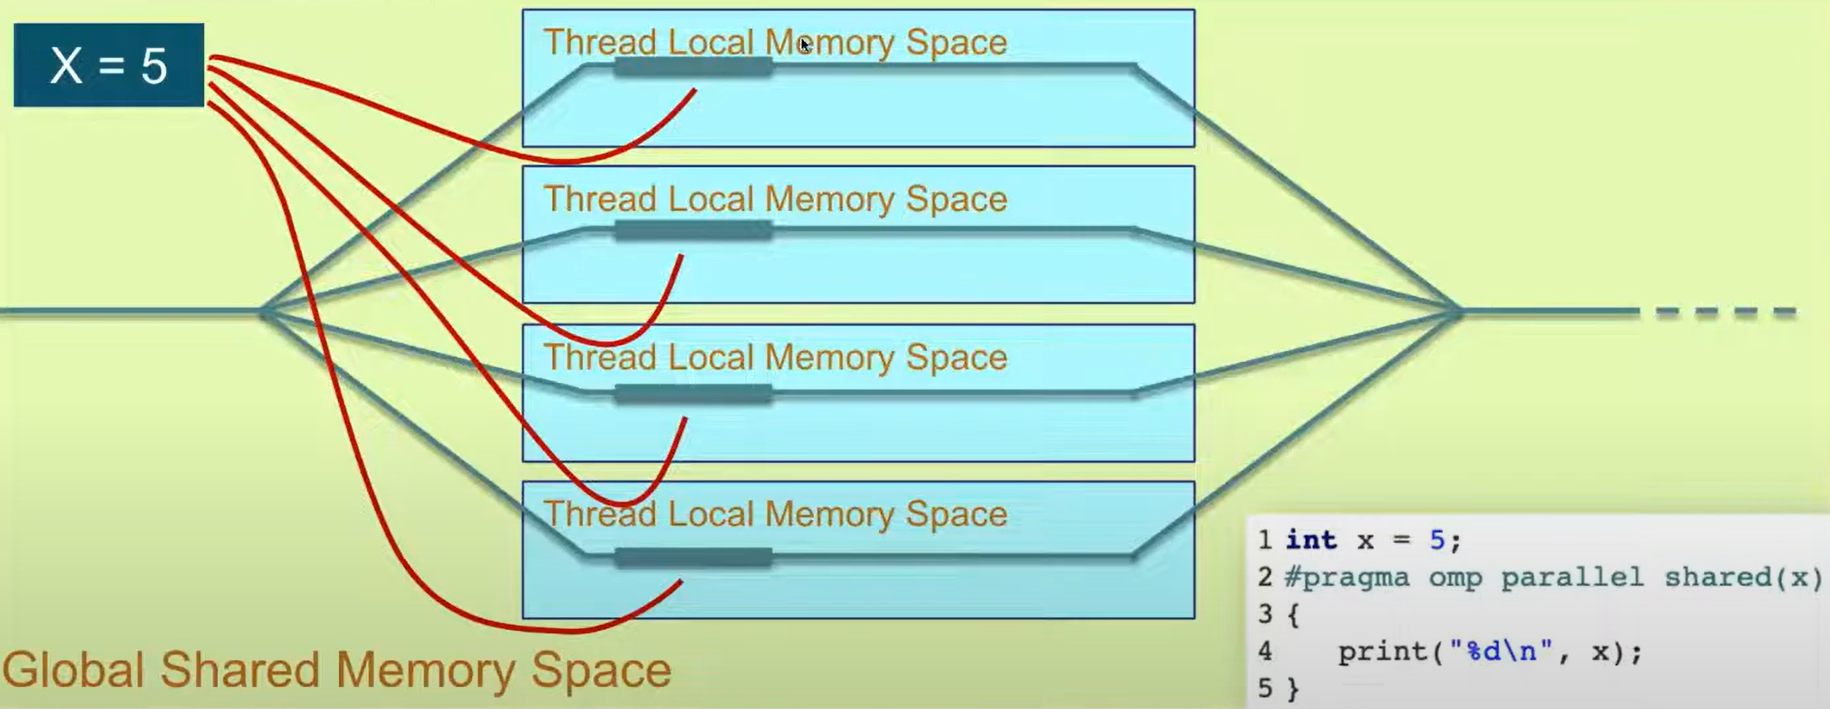
\includegraphics[width=\textwidth]{shared}    
\end{frame}


\begin{frame}[fragile]{Shared}
\lstset{language=C++}
  \begin{lstlisting}
#include <stdio.h>
#include <omp.h>


int main() {
    int i = 0;

    #pragma omp parallel shared(i) num_threads(10000)
    {
        i++;
    }

    printf("i = %d\n",i);
    return 0;
}    
  \end{lstlisting}
\end{frame}

\begin{frame}{Atomic}
  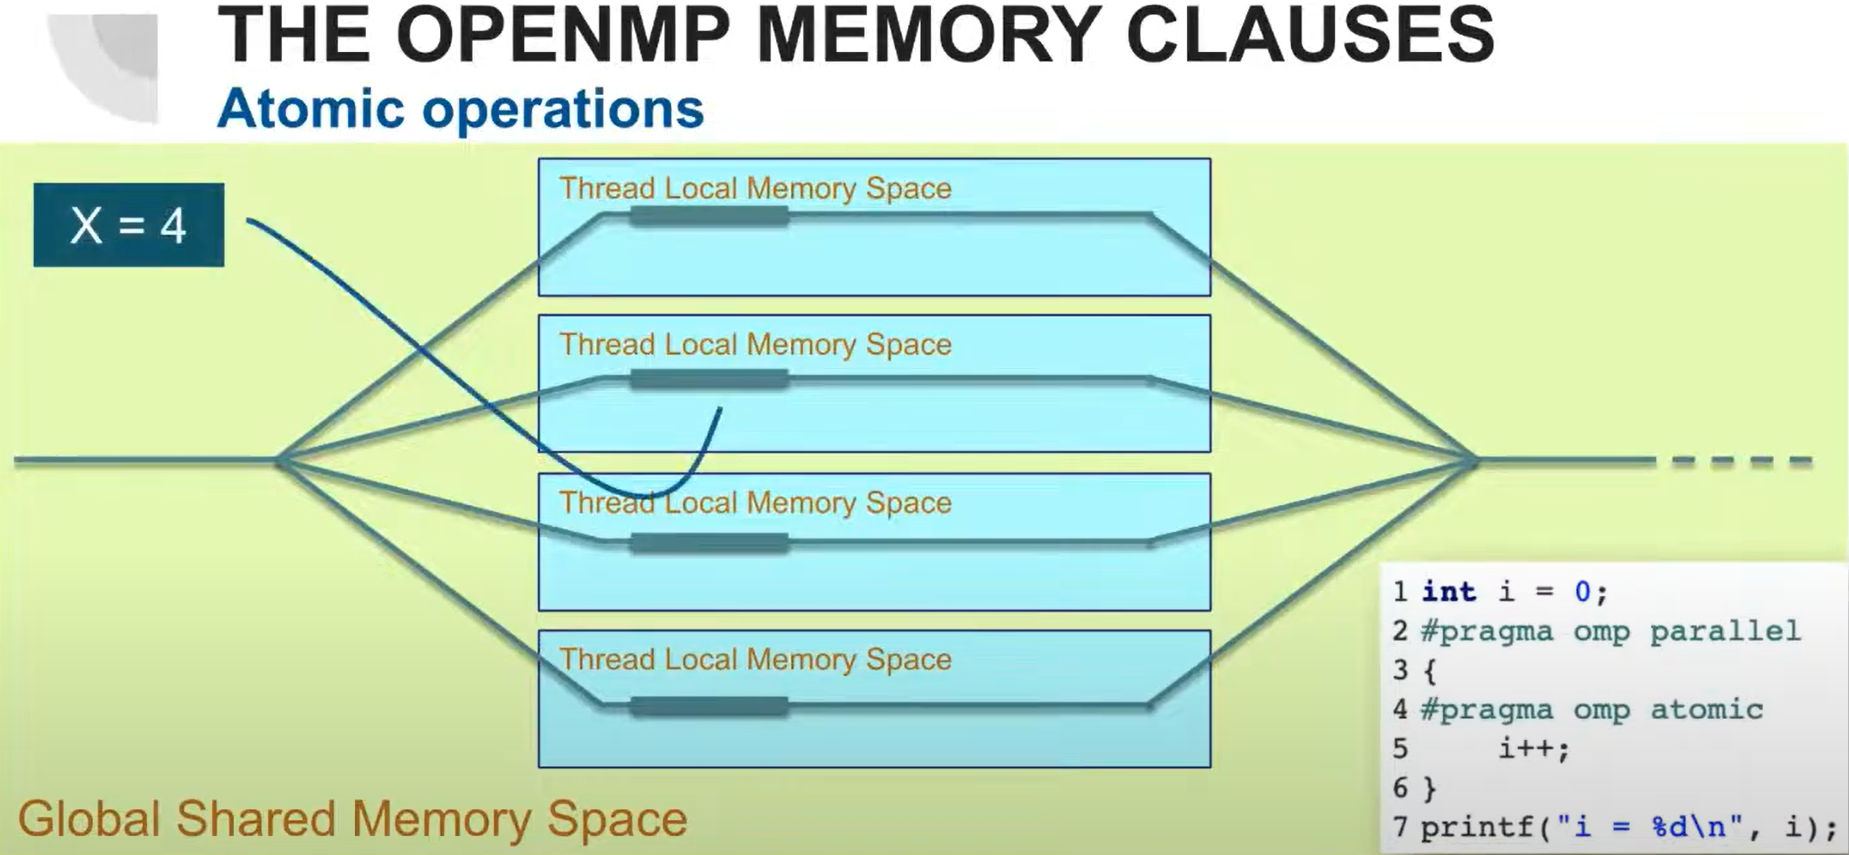
\includegraphics[width=\textwidth]{atomic}  
\end{frame}

\begin{frame}[fragile]{Atomic}
\lstset{language=C++}
  \begin{lstlisting}
#include <stdio.h>
#include <omp.h>


int main() {
    int i = 0;

    #pragma omp parallel shared(i) num_threads(10000)
    {
        #pragma omp atomic
        i++;
    }

    printf("i = %d\n",i);
    return 0;
}
  \end{lstlisting}
\end{frame}

\begin{frame}{Private}
  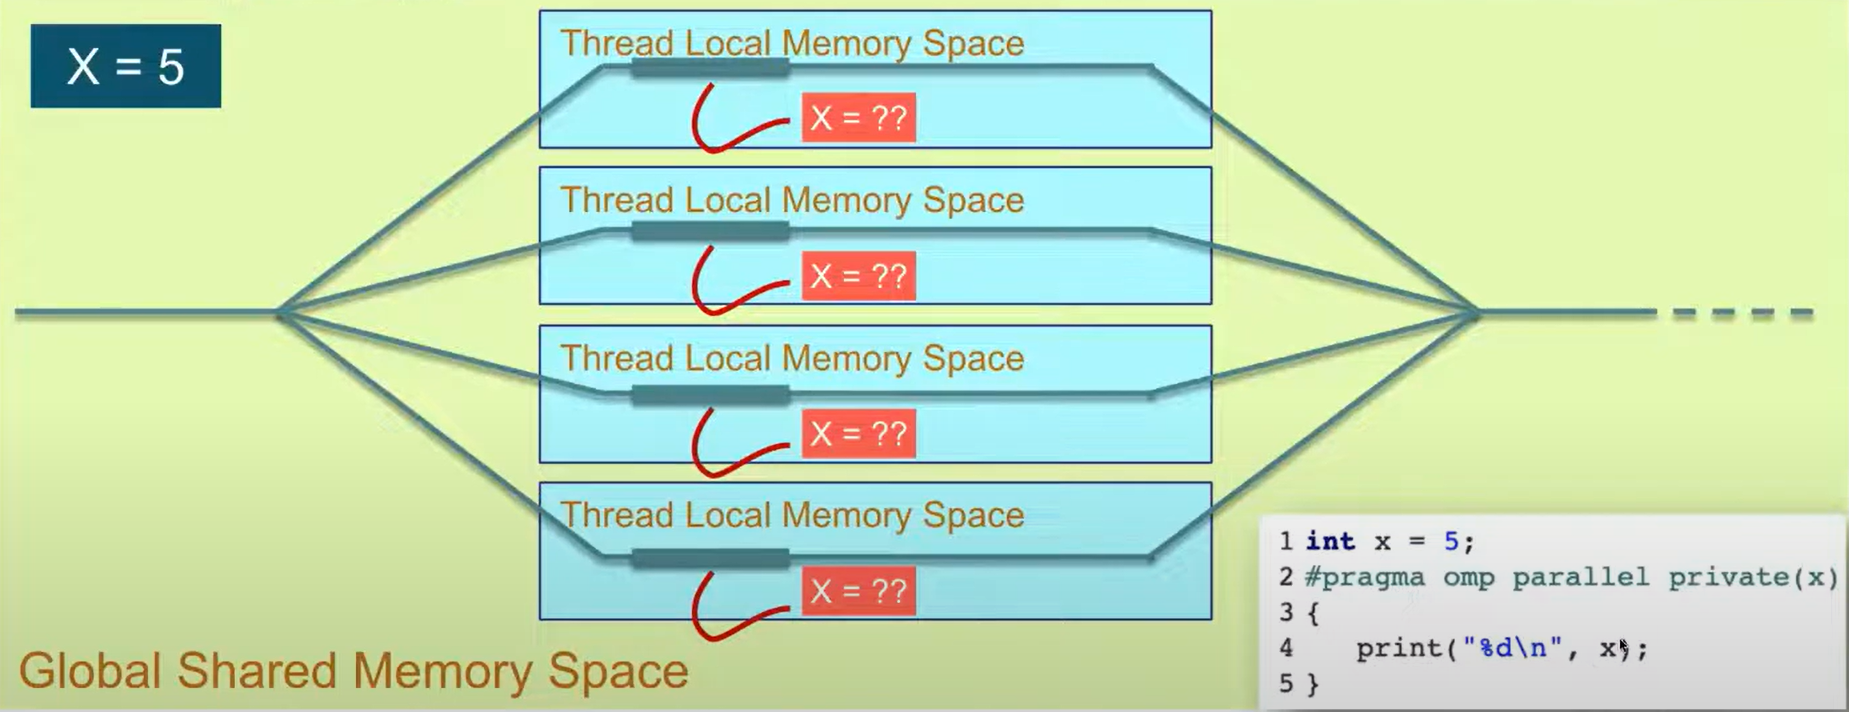
\includegraphics[width=\textwidth]{private}
\end{frame}

\begin{frame}[fragile]{Private}
\lstset{language=C++}
\begin{lstlisting}
#include <stdio.h>
#include <stdlib.h>
#include <omp.h>


int main() {
    int i = 999;

    printf("i is %d before parallel region\n",i);

    #pragma omp parallel private(i) num_threads(10)
    {
        printf("Thread %d sees %d on memory %lx\n", omp_get_thread_num(), i, (unsigned long)&i);
    }

    return 0;
}
  \end{lstlisting}
\end{frame}

\begin{frame}{Firstprivate}
  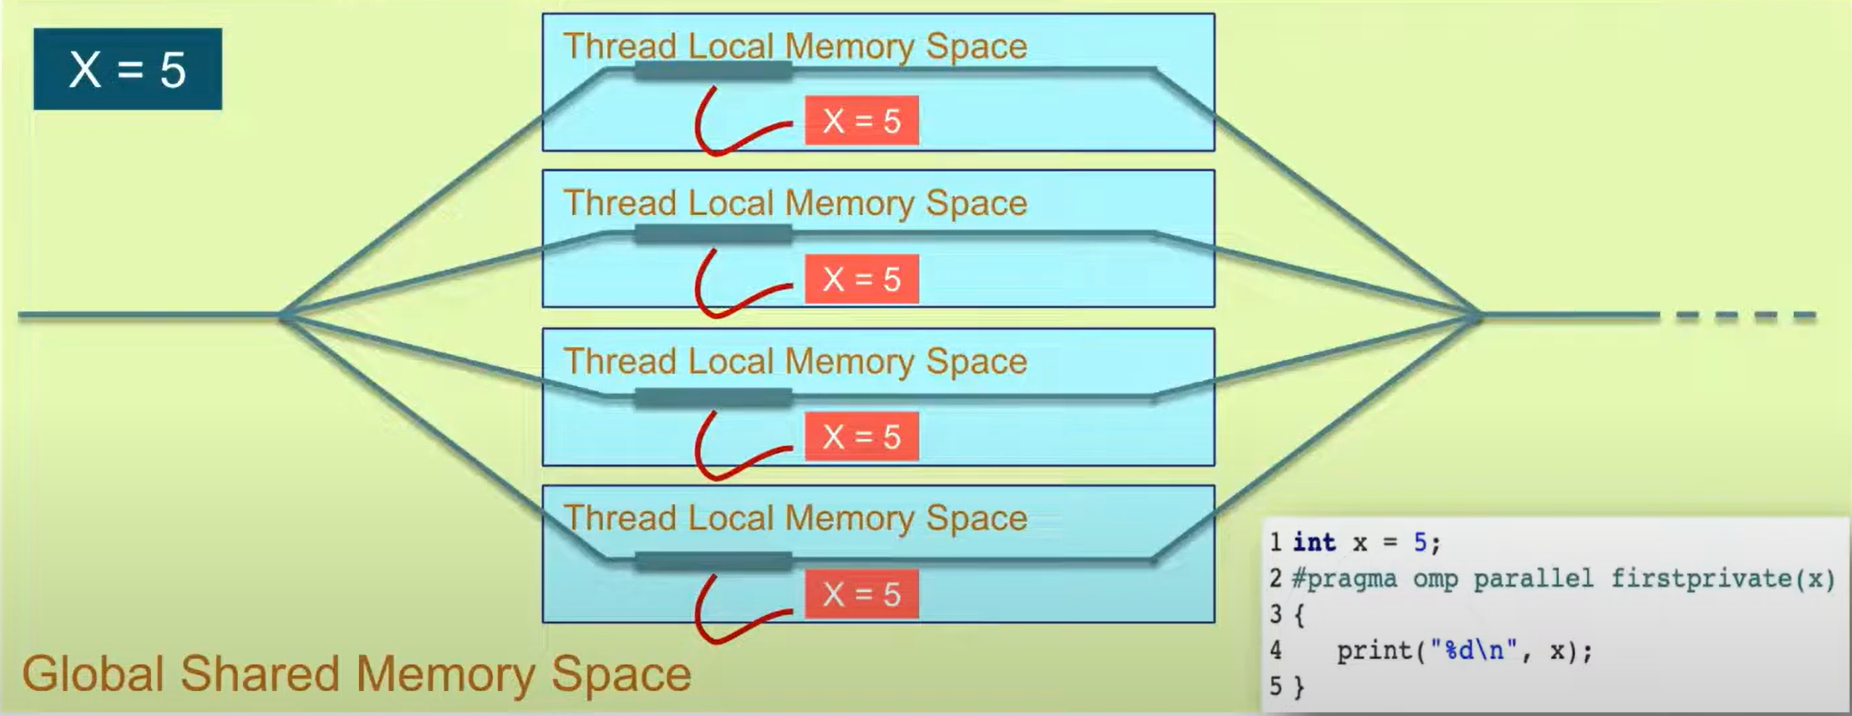
\includegraphics[width=\textwidth]{firstprivate}
\end{frame}

\begin{frame}[fragile]{Firstprivate}
\lstset{language=C++}
\begin{lstlisting}
#include <stdio.h>
#include <stdlib.h>
#include <omp.h>


int main() {
    int i[3] = {999,888,666};

    printf("i is [%d,%d,%d] before parallel region\n",i[0],i[1],i[2]);

    #pragma omp parallel firstprivate(i) num_threads(10)
    {
        printf("Thread %d sees [%d,%d,%d] on memory %lx\n", omp_get_thread_num(), i[0],i[1],i[2], (unsigned long)i);
    }

    return 0;
}
  \end{lstlisting}
\end{frame}


\begin{frame}[fragile]{Reduction}
  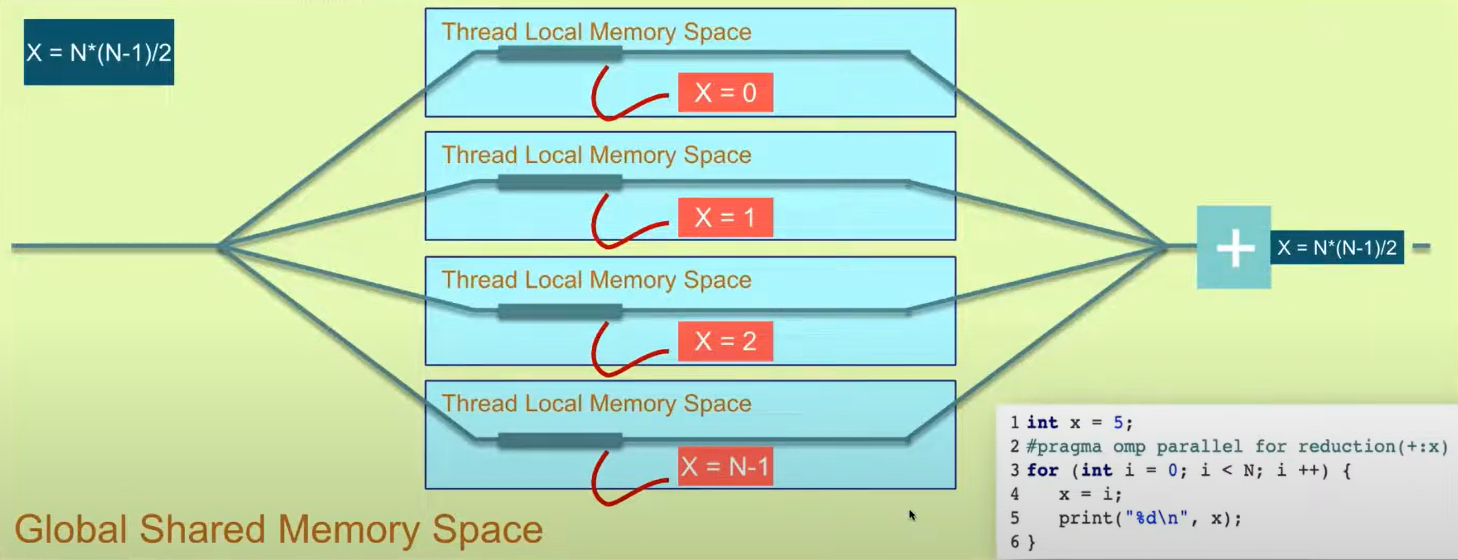
\includegraphics[width=\textwidth]{reduction}
\end{frame}

\begin{frame}[fragile]{Reduction}
\lstset{language=C++}
\begin{lstlisting}
#include <stdio.h>
#include <omp.h>


int main() {
    int i = 99;

    printf("Value if i prior to parallel region is %d\n",i);

    // Private values are not transferred back
    #pragma omp parallel private(i)
    {
        i=1000;
    }
    printf("Value if i after parallel region with private(i) is %d\n",i);

    i = 0;
    // Reductions for addition.
    #pragma omp parallel reduction(+:i) num_threads(10)
    {
        i=1;
    }
    printf("Value if i after parallel region with reduction(+:i) is %d\n",i);

    // Reductions for max.
    #pragma omp parallel reduction(max:i) num_threads(20)
    {
        i=omp_get_thread_num();
    }
    printf("Value if i after parallel region with reduction(max:i) is %d\n",i);

    return 0;
}
  \end{lstlisting}
\end{frame}

\begin{frame}[fragile]{Домашна работа}
  1. Прегледайте видеото на \url{https://www.youtube.com/watch?v=IsBgW7-yldA}.

  2. Компилирайте ``сорс''-овете от
  \url{https://github.com/josemonsalve2/openmp_tutorial/blob/main/Labs/Lab1/C}
  на \verb+neutronstar.iaps.institute+ или другаде.
\end{frame}


\begin{frame}{Реализация на OpenMP в различните компилатори}
  \url{https://www.openmp.org/resources/openmp-compilers-tools/}
\end{frame}


\begin{frame}{Синтаксис. Понятия.}
  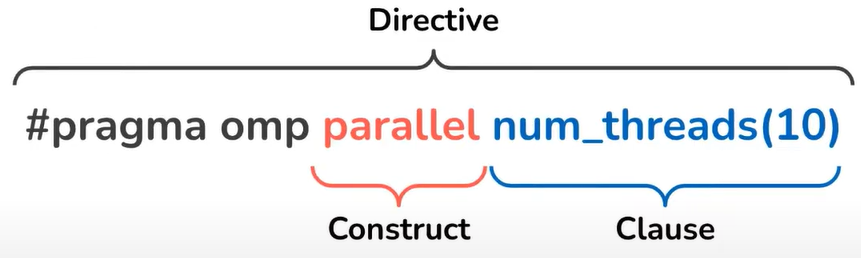
\includegraphics[width=\textwidth]{terms-pragma}
\end{frame}

\begin{frame}{Компилиране}
  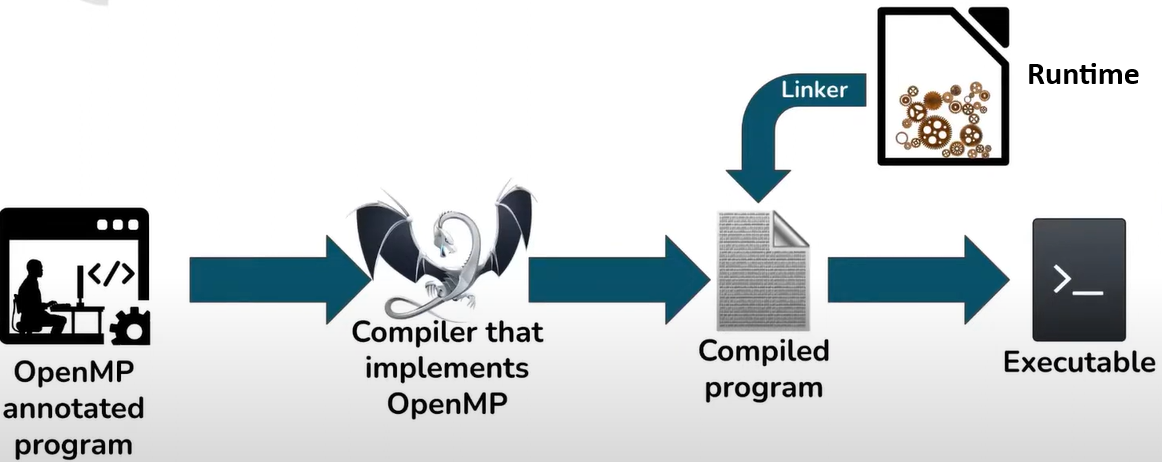
\includegraphics[width=\textwidth]{compilaton-process.png}
\end{frame}

\begin{frame}[fragile]{Function outlining}
  \lstset{language=C++}
\begin{lstlisting}
  #pragma omp parallel{
    printf("hello world\n");
  }
\end{lstlisting}

\begin{lstlisting}
  void outlined_function(void* params)
  {
    printf("hello world\n");
  }

  __runtime_omp_parallel(outlined_function, params);
\end{lstlisting}

\end{frame}

\end{document}

%%% Local Variables:
%%% mode: latex
%%% TeX-master: t
%%% End:
